\section{Week 5}
\textbf{\large $\mathcal{Z}$-plane stability:}
\vspace{0.4cm}


\textbf{\underline{Case 1: z is real}}
\begin{figure}[H]
    \centering
    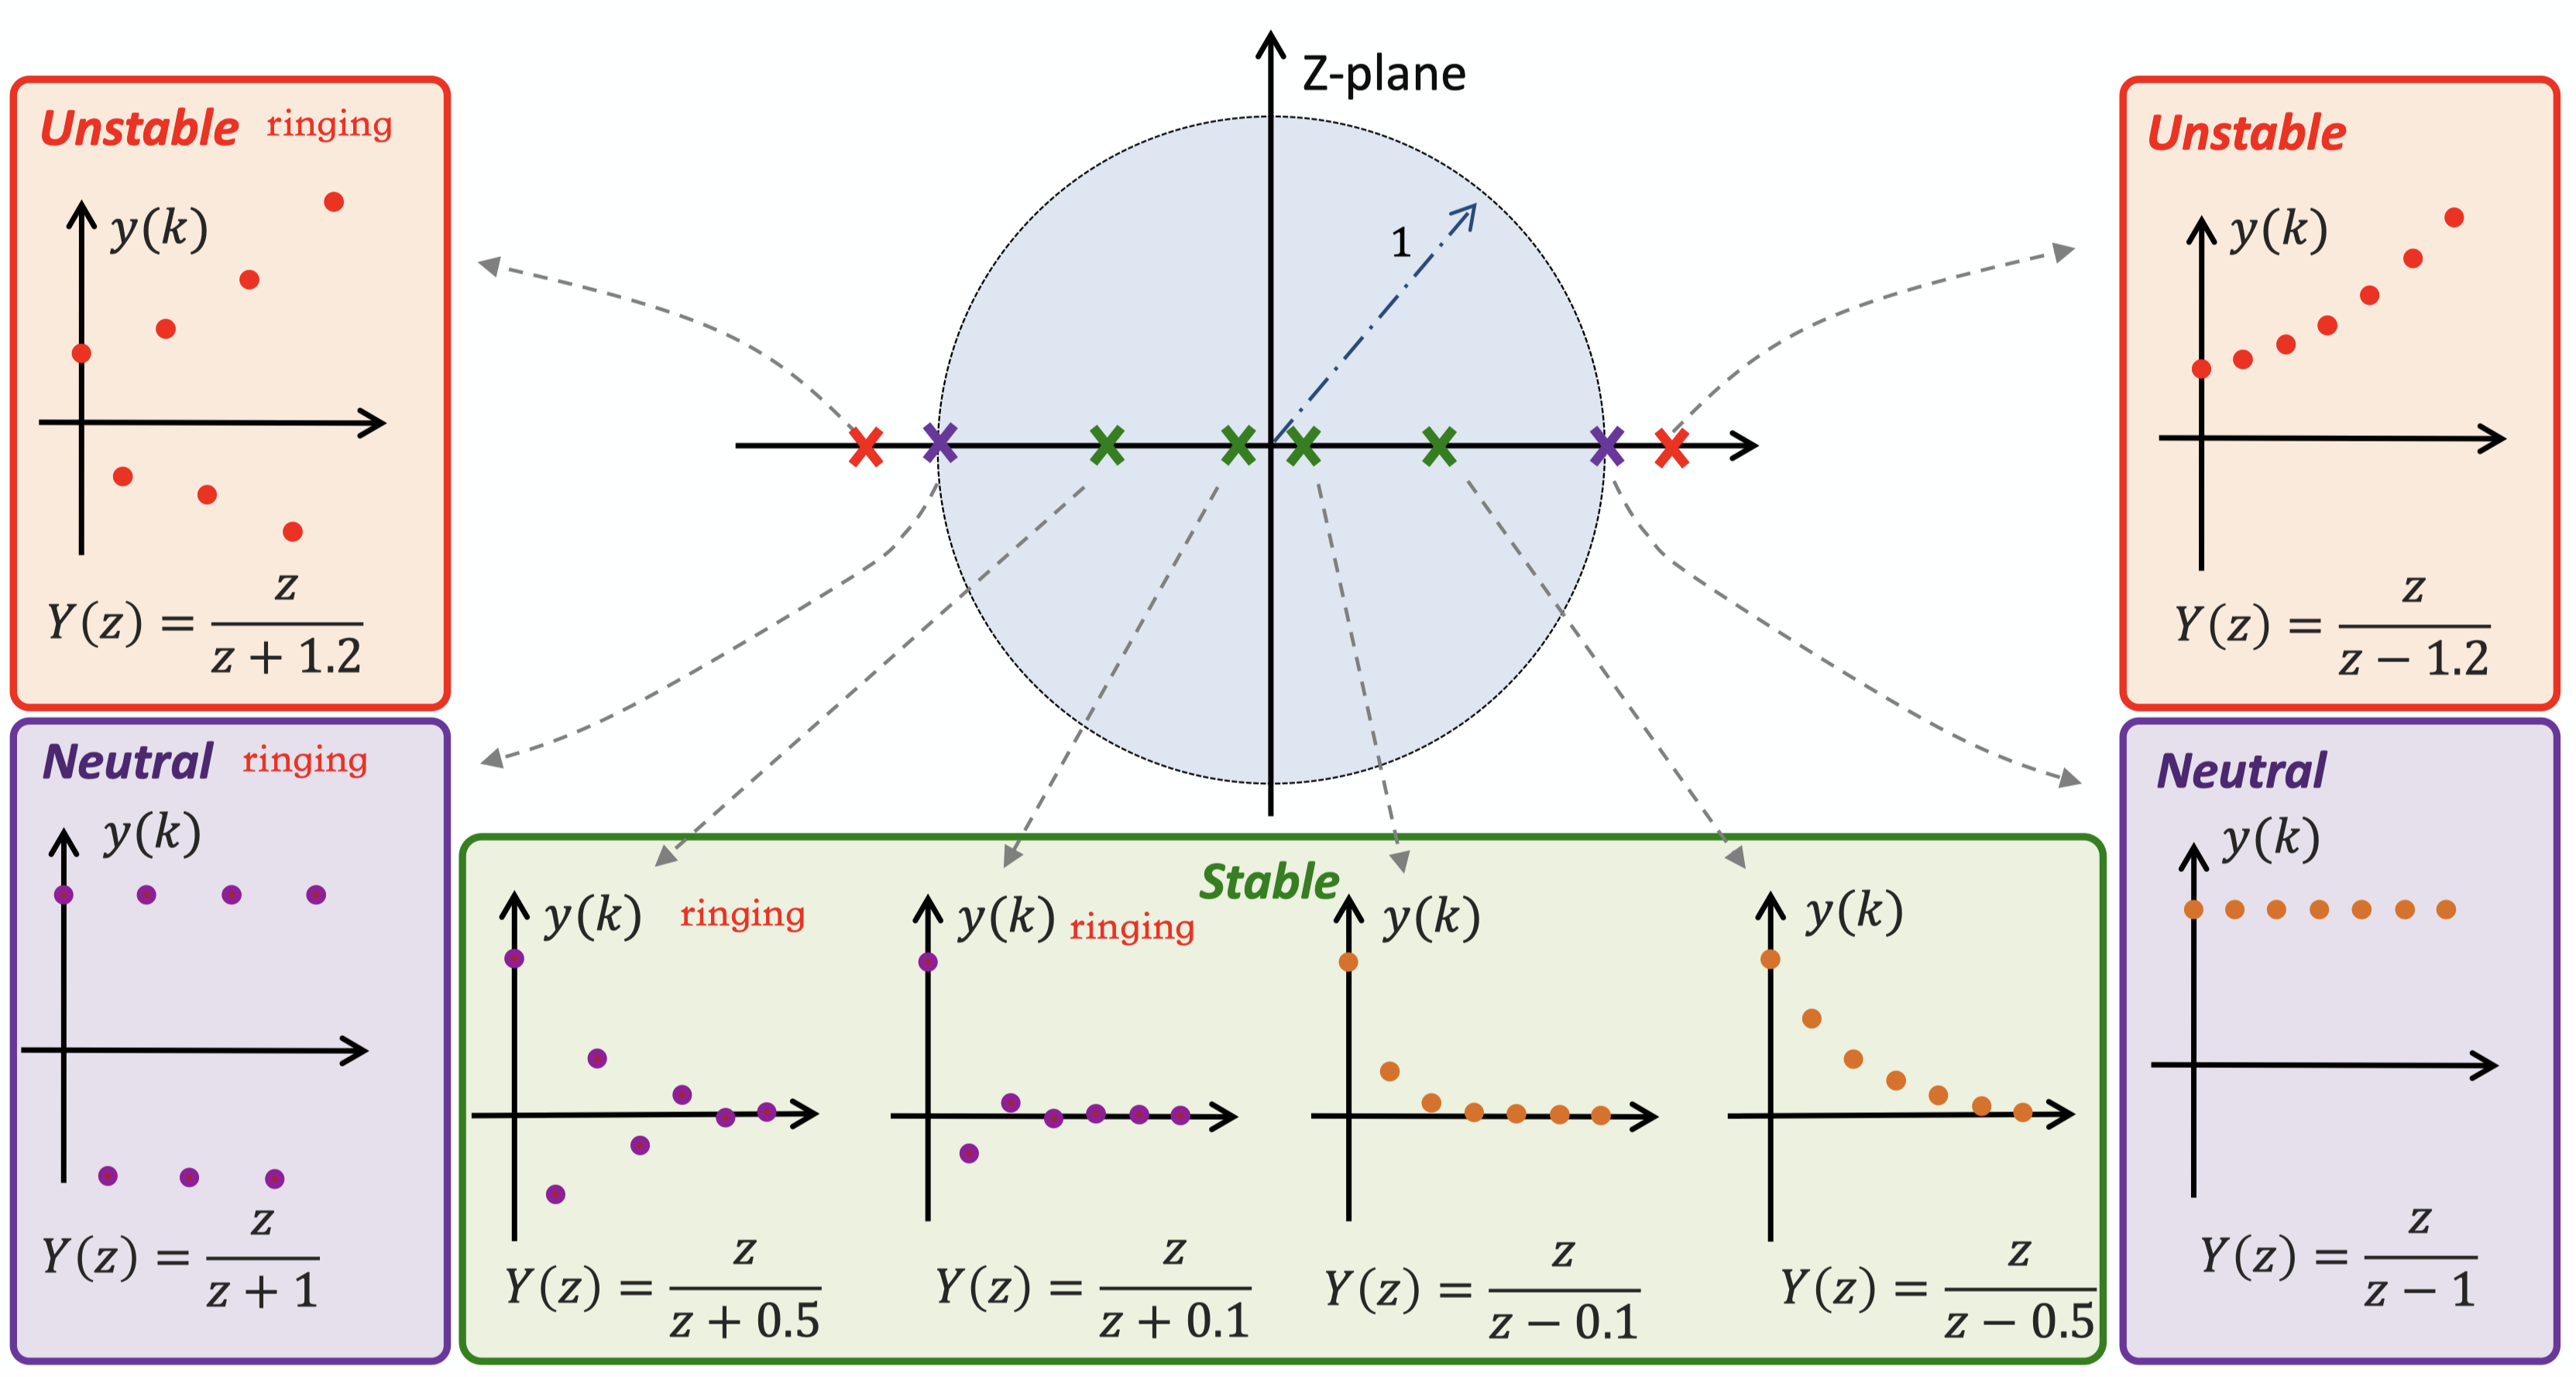
\includegraphics[width=0.5\textwidth]{images/z_plane_stability.png}
\end{figure}

\begin{table}[h]
\begin{adjustbox}{max width=\textwidth}
\begin{tabular}{|c|p{0.2\textwidth}|c|c|}
\hline
\textbf{$z=a$} & \textbf{transient response} & \textbf{stability} & \textbf{ringing?} \\\hline
$a> 1$ & transient term will grow & unstable & No \\\hline
$a = 1$ & transient term will remain constant & neutral & No \\\hline
$0<a<1$ & transient term will die down & stable & No \\\hline
$a=0$ & transient term will disappear in one sampling interval & stable & No \\\hline
$-1<a<0$ & transient term will disappear & stable & Yes \\\hline
$a = -1$ & transient term will ring with constant amplitude & neutral & Yes \\\hline
$a < -1$ & transient term will ring and grow & unstable & Yes \\\hline
\end{tabular}
\end{adjustbox}
\end{table}

\textbf{\underline{Case 2: z is complex}}
\begin{table}[h]
\begin{adjustbox}{max width=\textwidth}
\begin{tabular}{|c|c|c|}
\hline
\textbf{$z=p\pm jq = re^{\pm j\theta}$} & \textbf{$Cr^k \cos(k\theta + \phi)$} & \textbf{stability} \\\hline
$r\ge 1$ & oscillatory, grow to $\infty$ & unstable \\\hline
$r=1$ & oscillatory, stay steady & neutral $a=-1$ \\\hline
$0<r<1$ & oscillatory, disappear as $t\to\infty$ & stable  \\\hline
$r=0$ & disappear in one sample interval & stable \\\hline
\end{tabular}
\end{adjustbox}
\end{table}

\textbf{\large Important Difference between s- and z-plane:} 
\begin{itemize}
    \item Double poles on the unit circle (a ramp) is not stable!
    \item System stable in s-domain for all value of $K$ is NOT necessarily stable in z-domain for all $K$ for certain sampling time $T$. Example: Kahoot wk7 Q9.
\end{itemize}

\textbf{\large $\mathcal{S}$-plane and $\mathcal{Z}$-plane Mapping}
\begin{equation*}
    s= e^{Ts} = e^{T(\sigma + j \omega)} = e^{T\omega} e^{T j\omega} = r e^{T j\omega}
\end{equation*}
N.B. not sure if $T$ should be included, since $T$ does not influence the plots in both s-domain and z-domain.
\begin{align*}
    s &= \sigma + j \omega_d \; \begin{cases}
    \sigma = \frac{\ln(r)}{T}\; , & |z| = r = e^{\sigma} \\
    \omega_d = \frac{\theta}{T} \; , & \angle z = \omega_d 
    \end{cases} \\
    C_0 &= -\frac{\sigma}{\omega} = - \frac{\ln(r)}{\theta} = -\sqrt{\frac{\zeta}{1-\zeta^2}} 
\end{align*}
\begin{figure}[H]
    \centering
    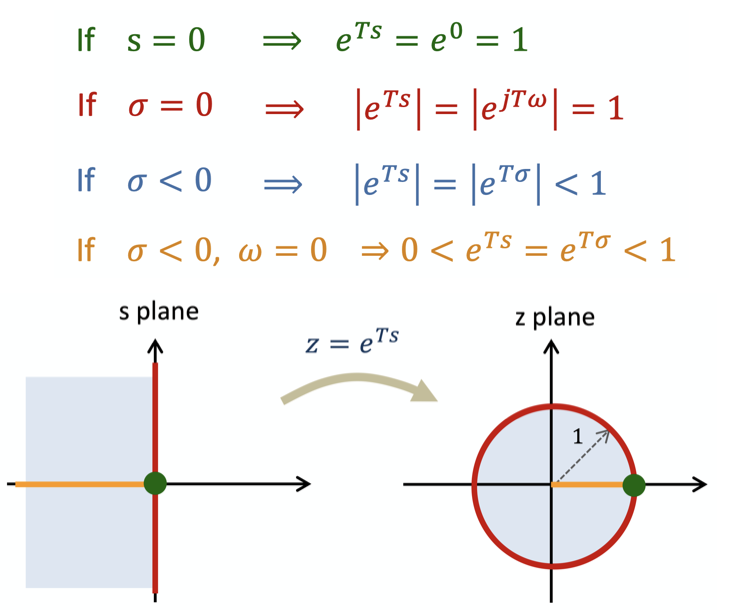
\includegraphics[width=0.5\textwidth]{images/s_z_mapping.png}
\end{figure}

\textbf{\underline{Critical Points:}}
\begin{itemize}
    \item Origin $s=0$ mapped to $z=e^0 = 1$ (real axis);
    \item Constant settling time / vertical line / $Re(s)=\sigma$ mapped to a circle $|z|=e^{\sigma}$ centered at origin:
    \begin{itemize}
        \item Line $Re(s)=-\infty$ mapped as the origin since $|z|=e^{-\infty}=0$;
        \item Im axis $Re(s)=0$ mapped as the unit circle since $|z|=e^0=1$;
        \item Line $Re(s)=\infty$ mapped as the circle of infinite radius since $|z|=e^{\infty}=\infty$.
    \end{itemize}
    \item Constant frequency line / horizontal line / $Im(s)=j\omega_d$ mapped as a ray starting from the origin with angle $\angle \omega_d$ ;
    \item The range $\omega_d \in (-\infty, \infty)$ is mapped to a finite range $\omega_d \in [0, 2\pi]$.
\end{itemize}

\begin{figure}[H]
    \centering
    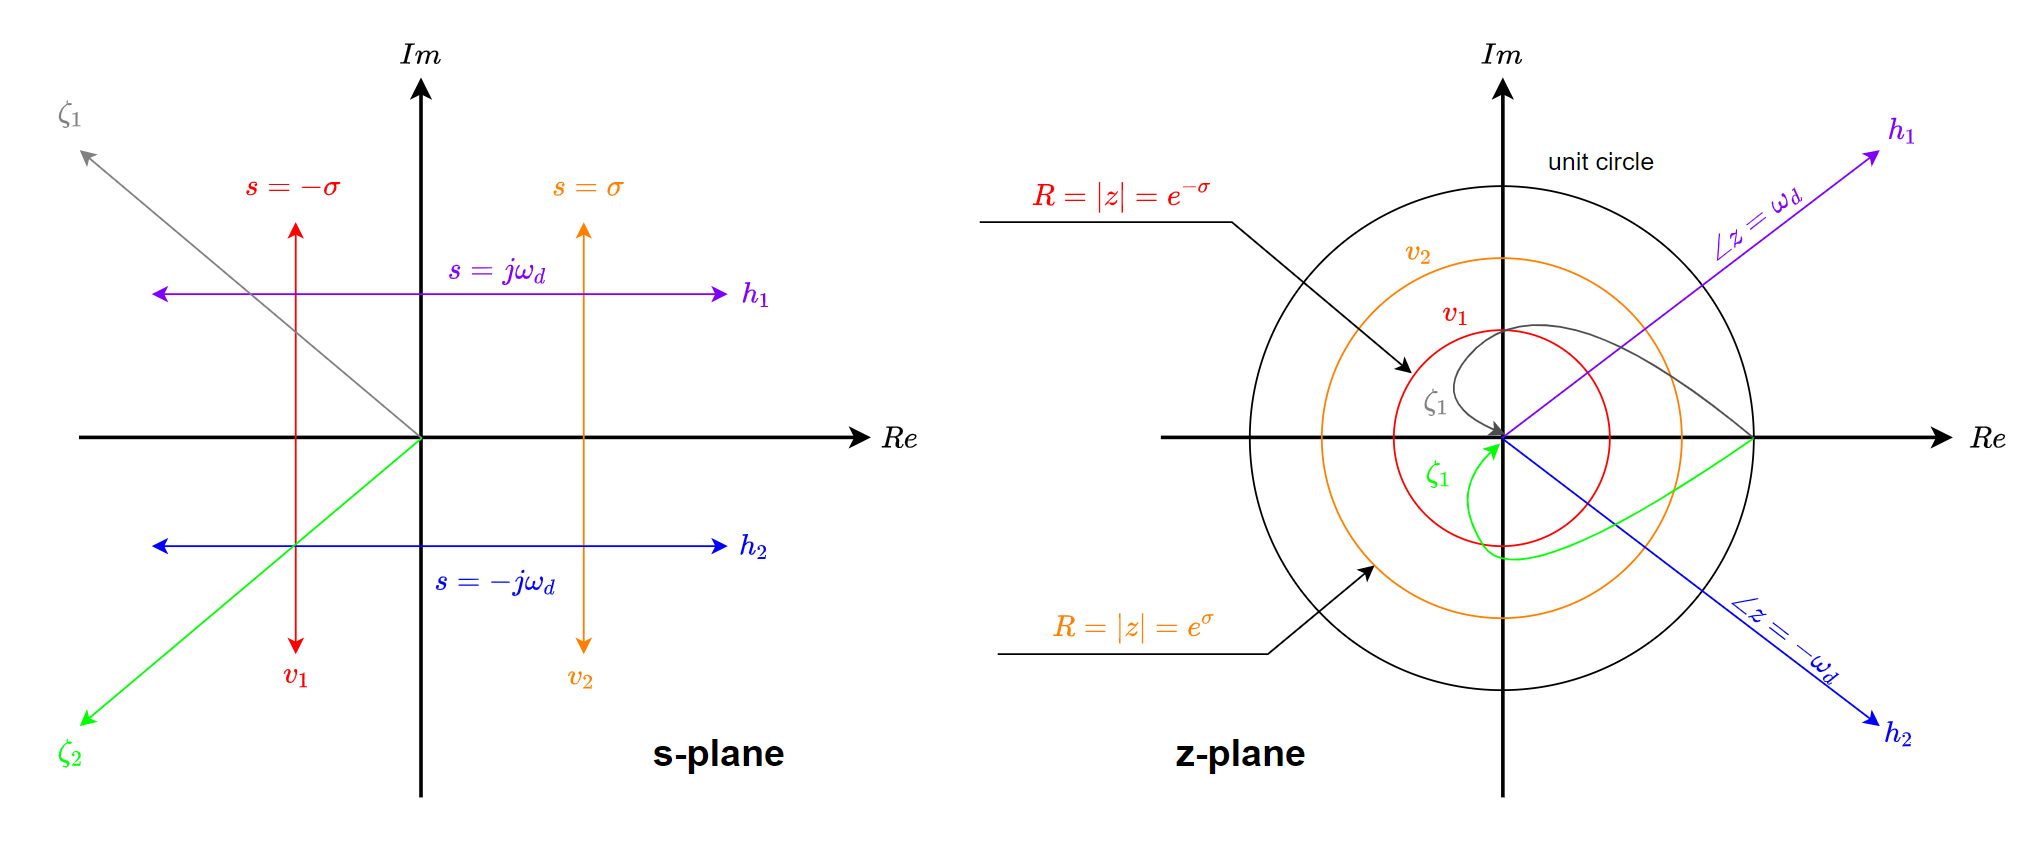
\includegraphics[width=1.0\linewidth]{images/Mapping_sumary_1.png}
\end{figure}
\begin{figure}[H]
    \centering
    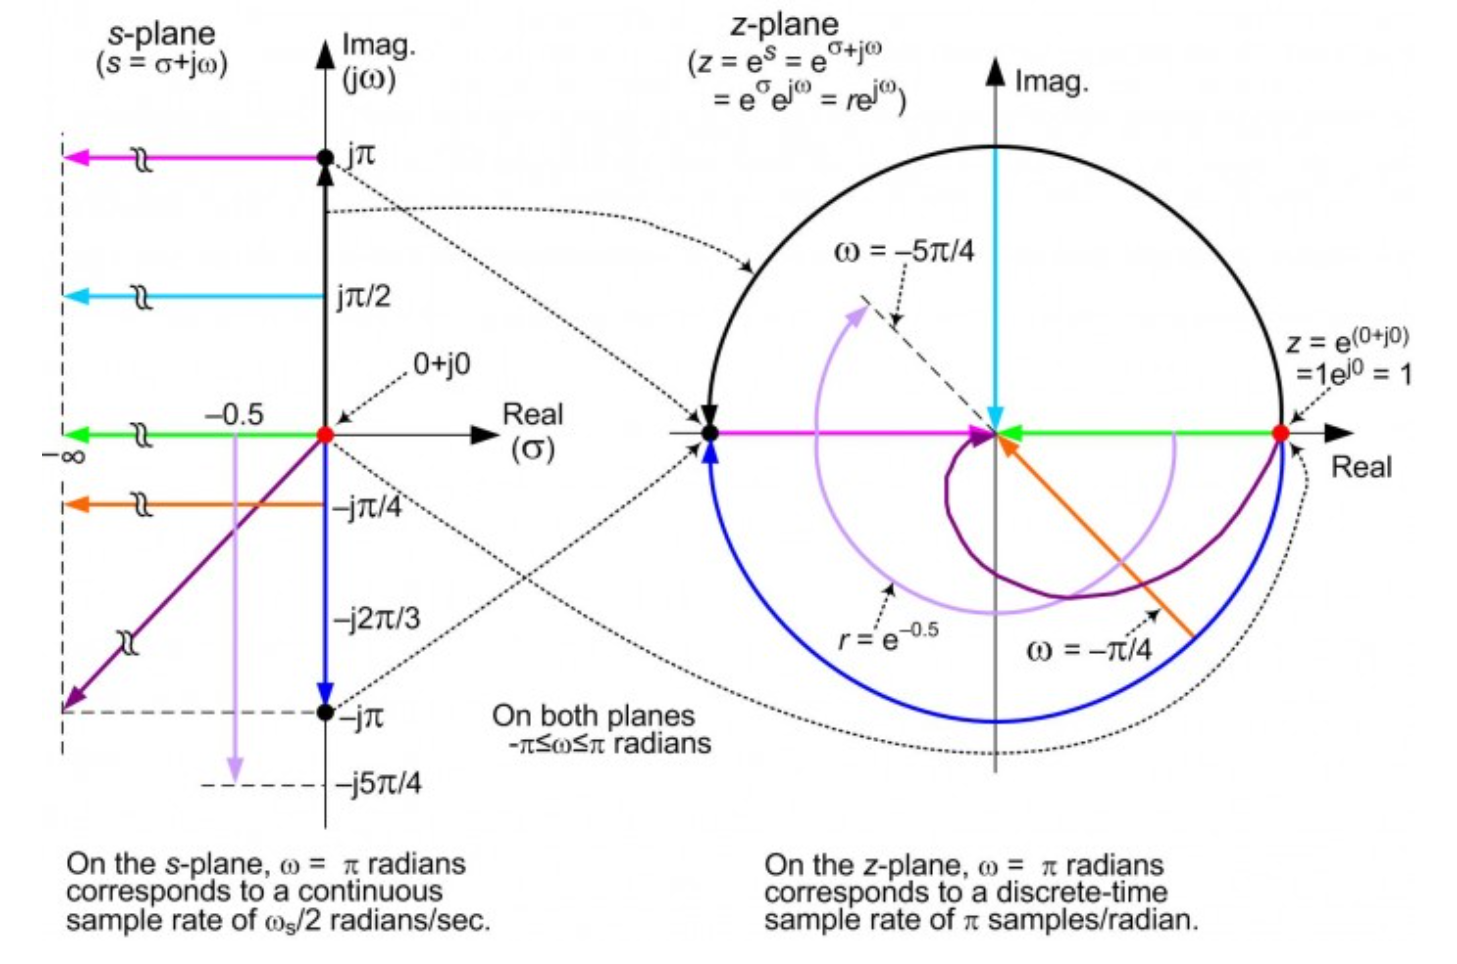
\includegraphics[width=1.0\linewidth]{images/Mapping_sumary_2.png}
\end{figure}

\textbf{\large Dominant poles in z-plane}: 
\begin{itemize}
    \item The poles closer to the unit circle are the dominant/slowest poles.
\end{itemize}


\textbf{\large Steady state gains}
\begin{itemize}
    \item \textbf{DC Gain} = $\lim_{z\to 1} G(z)$ 
    \item \textbf{Inst. Gain} = $\lim_{z\to \infty} G(z)$
\end{itemize}

\textbf{\large Discrete State Space}
\begin{equation*}
    \begin{cases}
     \dot{x}(t) = \bm{A}x(t) + \bm{B}u(t) \\
     y(t) = \bm{C}x(t)+\bm{D} u(t)
    \end{cases}, \; \begin{cases}
     x(k+1) = \bm{G}x(k) + \bm{H}u(k) \\
     y(kT) = \bm{C}x(kT) + \bm{D}u(kT)
    \end{cases}
\end{equation*}
\begin{align*}
    \text{where } \bm{G} &= e^{\bm{A}T} \\
    \bm{H} &= \int_{0}^{T}\left(e^{\bm{A}\lambda} d\lambda\right) \bm{B} \\
    &= \bm{A}^{-1} (e^{\bm{A}T}- \bm{I})\bm{B}
\end{align*}

\textbf{From z-pole to $\bm{\omega_d}$:}

\begin{enumerate}
    \item Given that $z=a+j\, b$, $T$ is known,
    \item From $z=e^{sT}$ we have $s=\frac{\ln(a+j\, b)}{T}=\sigma + j\, \omega_d$
\end{enumerate}

\textbf{From z-pole to 95\% $\bm{t_s}$:}
\begin{enumerate}
    \item $s = \frac{\ln(z)}{T} = \sigma + j\,\omega_d$ ,
    \item $e^{\sigma \, t_s} = 1 - 0.95$,
    \item $t_s = \frac{\ln(1-0.95)}{\sigma}\;$, ($t_s$ should be +ve).
\end{enumerate}